\documentclass[a4paper,11pt]{article}
\usepackage[utf8]{inputenc}
\usepackage[T1]{fontenc}
\usepackage{graphicx}
\usepackage[T2A]{fontenc}
\usepackage[utf8]{inputenc}
\usepackage[english]{babel}
\usepackage{extsizes}
\usepackage{indentfirst}
\usepackage{fancyhdr}
\usepackage{geometry}
\usepackage{amsthm}
\usepackage{amsfonts}
\usepackage{mathtools}
\usepackage{graphicx}
\usepackage{wrapfig}
\usepackage{caption}
\usepackage{amssymb}
\usepackage{booktabs}
\usepackage{dsfont}
\usepackage[toc,page]{appendix}
\usepackage[export]{adjustbox}
\usepackage[percent]{overpic}

\theoremstyle{plain}
\newtheorem{thm}{Theorem}[part]% reset theorem numbering for each part
\newtheorem{lmm}[thm]{Lemma}
\newtheorem{crlr}[thm]{Corollary}

\theoremstyle{definition}
\newtheorem{defn}[thm]{Definition}
\newtheorem{exmp}[thm]{Example}
\newtheorem{rmrk}[thm]{Remark}
\newtheorem{asmp}[thm]{Assumptions}
\newtheorem{prps}[thm]{Proposition}
\newtheorem{cond}[thm]{Conditions}

\renewcommand{\theenumi}{\roman{enumi}}
\renewcommand{\labelenumi}{(\theenumi)}
\renewcommand\thepart{\arabic{part}}

\newcommand{\ME}{\mathbb{E}}
\newcommand{\MR}{\mathbb{R}}
\newcommand{\MP}{\mathbb{P}}
\newcommand{\MN}{\mathbb{N}}
\newcommand{\Var}{\operatorname{Var}}
\newcommand{\Cov}{\operatornamerm{Cov}}
\newcommand{\diag}{\operatorname{diag}}
\newcommand{\tr}{\operatorname{tr}}
\newcommand{\convdistr}{\xrightarrow{\mathcal{L}}}
\newcommand{\convprob}{\xrightarrow{\MP}}
\newcommand{\define}[1]{\textit{\textbf{#1}}}

\title{On the estimation of spectral distribution of integrated covariance matrices of high dimensional stochastic processes}
\author{Aleksandr Samarin}
\date{August 2017}

\begin{document}
	\maketitle
	
	\begin{abstract}
		In the 1-subject Master's program in Financial Mathematics of the Faculty of Mathematics and Natural Sciences of the CAU in Kiel
		
		presented by Aleksandr Samarin
		
		First referee:
		Second referee:
		Kiel, August 2017
		
		(COPIED FROM THE PAPER) \\
		We consider the estimation of integrated covariance (ICV) matrices
		of high dimensional diffusion processes based on high frequency
		observations. We start by studying the most commonly used estimator,
		the realized covariance (RCV) matrix. We show that in the
		high dimensional case when the dimension p and the observation frequency
		n grow in the same rate, the limiting spectral distribution
		(LSD) of RCV depends on the covolatility process not only through
		the targeting ICV, but also on how the covolatility process varies in
		time. We establish a Marcenko–Pastur type theorem for weighted
		sample covariance matrices, based on which we obtain a Marcenko–
		Pastur type theorem for RCV for a class C of diffusion processes.
		The results explicitly demonstrate how the time variability of the
		covolatility process affects the LSD of RCV. We further propose
		an alternative estimator, the time-variation adjusted realized covariance
		(TVARCV) matrix. We show that for processes in class C, the
		TVARCV possesses the desirable property that its LSD depends
		solely on that of the targeting ICV through the Marcenko–Pastur
		equation, and hence, in particular, the TVARCV can be used to recover
		the empirical spectral distribution of the ICV by using existing
		algorithms
	\end{abstract}
	
	\pagebreak
	\tableofcontents
	
	\pagebreak
	\part{Introduction}
	
	\section*{Motivation}
    Say general words...  v
    
    Suppose that we have multiple stocks, say, $p$ stocks, whose log price processes are denoted by $X_t^{(j)}$ for $j = 1, \dots, p$. Let
	\[ \mathbf{X}_t = \big(X_t^{(1)}, \dots, X_t^{(p)}\big)^T. \]
	Then a widely used model for $\mathbf{X}_t$ is
	\begin{equation} \label{X diffeq}
		d\mathbf{X}_t = \boldsymbol{\mu}_t dt + \Theta_td\mathbf{W}_t,
	\end{equation}
	where 
	\begin{itemize}
		\item $\boldsymbol{\mu}_t = (\mu_t^{(1)}, \dots, \mu_t^{(p)})^T$ is a $p$-dimensional drift process,
		\item $\Theta_t$ -- $p \times p$ \define{covolatility process},
		\item $\mathbf{W}_t$ -- $p$-dimensional standard Brownian motion.
	\end{itemize}


	\begin{defn} \
		\begin{enumerate}
			\item The \define{integrated covariance matrix (ICV)} is defined as follows
			\[\Sigma_p := \int_0^1\Theta_t \Theta_t^T dt.\]
			For $p=1$ ICV is called \define{integrated volatility}.
			\item Set time points $ \{\tau_\ell\}_{0 \leq \ell \leq n}$. Then \define{realized covariance (RCV)} is
			\begin{equation} \label{RCV}
				\Sigma_p^{RCV} := \sum_{\ell=1}^{n}\Delta \mathbf{X}_\ell(\Delta \mathbf{X}_\ell)^T,
			\end{equation}
			where 
			\[ \Delta \mathbf{X}_\ell :=
			\begin{pmatrix}
			\Delta X_\ell^{(1)} \\
			\vdots \\
			\Delta X_\ell^{(p)}
			\end{pmatrix}
			=
			\begin{pmatrix}
			X_{\tau_{\ell}}^{(1)} - X_{\tau_{\ell-1}}^{(1)} \\
			\vdots \\
			X_{\tau_{\ell}}^{(p)} - X_{\tau_{\ell-1}}^{(p)}
			\end{pmatrix}. \]
			For $p=1$ RCV is called \define{realized volatility}.
		\end{enumerate}
	\end{defn}
	
	\begin{exmp} \label{exmp X3}
		(CHECK NON-SYMMETRIC THETA) Let's take $p = 3$, zero drift $\mu_t = (0, 0, 0)^T$ and 
		\[ \Theta_t = \begin{pmatrix}
		1 & \cos(\pi t) & \sin (\pi t) \\
		\cos(\pi t) & 1 & 0 \\
		\sin (\pi t) & 0 & 1
		\end{pmatrix}. \]
		Then 
		\[ \Theta_t\Theta_t^T = \begin{pmatrix}
		2 & 2\cos(\pi t) & 2\sin (\pi t) \\
		2\cos(\pi t) & \cos^2(\pi t) + 1 & \cos(\pi t)\sin(\pi t) \\
		2\sin (\pi t) & \cos(\pi t)\sin(\pi t) & \sin^2(\pi t)+1
		\end{pmatrix} \]
		and corresponding ICV matrix is
		\[ \Sigma_3 = \begin{pmatrix}
		2 & 0 & \frac{4}{\pi} \\
		0 & \frac{3}{2} & 0 \\
		\frac{4}{\pi} & 0 & \frac{3}{2}
		\end{pmatrix}. \]
	\end{exmp}
	
	\begin{rmrk} \
		\begin{enumerate}
			\item 
			Intuitively, one can wish zero elements of the matrix $\Sigma_3$ from Example \ref{exmp X3} to show the independence of one process from another, or at least lack of correlation between them. But even if in the case of $(X_t^{(2)}, X_t^{(3)})$ it is true, it is totally wrong for $(X_t^{(1)}, X_t^{(2)})$. In this paper we focus on the processes, which correlation structure doesn't change in time. (SOMETHING ABOUT INTRADAY DATA)
			\item One of the major problems in of all the models, based on the theory of stochastic calculus and applied to financial markets, is the estimation of so-called true covariance. In our case the final goal is to find an estimator of an ICV matrix. In the next section we show how RCV matrix does the job.
		\end{enumerate}
	\end{rmrk}
	
	\begin{figure}
		\begin{center} \centering
			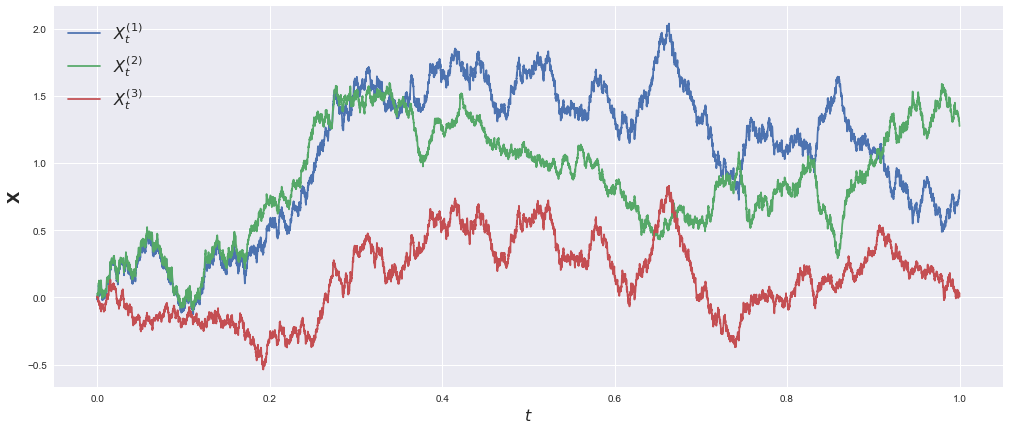
\includegraphics[scale=0.4]{X3}
			\caption{$\mathbf{X}_t$ from Example \ref{exmp X3}}
			\smallskip
			\small
			One can observe that $X_t^{(1)}$ and $X_t^{(2)}$ have strong positive correlation in the beginning, which decreases over time and later, when $t$ approaches $1$, turns into negative one. Meanwhile $X_t^{(3)}$ has independent fluctuations on the borders, but in the middle it repeats the behavior of $X_t^{(1)}$.
		\end{center}
	\end{figure}
	
	\section*{The relation between RCV and ICV}
	
	\begin{rmrk} \label{stoch calc notions}
		Recall the basic notions from the theory of stochastic calculus (w.l.o.g. we assume that all the processes have a starting point at $0$ a.s.):
		\begin{enumerate}
			\item An \define{Itô process} $X_t$ is defined to be an adapted stochastic process that can be expressed as the sum of an integral with respect to time and an integral with respect to Brownian motion:
			\[ X_t = \int_{0}^{t} \mu_s ds + \int_{0}^{t} \sigma_s dW_s. \]
			\item Let $X$ be a continuous local martingale. Then $[X]_t$ with
			\[ [X]_t = X_t^2 - 2 \int_0^t X_sdX_s \]
			is called \define{quadratic variation} of $X$.
			\item The \define{quadratic covariation} of two continuous semimartingales $X$ and $Y$ is defined as follows:
			\[ [X, Y]_t = \frac{1}{4}([X + Y]_t - [X-Y]_t). \]
			\item Let $X$ and $Y$ be Itô processes with volatilities ${\sigma_X}_t$ and ${\sigma_Y}_t$ with respect to the same Brownian motion, then
			\[ [X, Y]_t = \int_0^t {\sigma_X}_s{\sigma_Y}_s ds. \]
			\item Quadratic covariation is symmetric and bilinear map:
			\[ [X + Y, Z]_t = [X, Z]_t + [Y, Z]_t, \]
			\[ [X, Y + Z]_t = [X, Y]_t + [X, Z]_t, \]
			\[ [X, Y]_t = [Y, X]_t, \quad [X]_t = [X, X]_t \]
		\end{enumerate}
	\end{rmrk}
	
	\begin{exmp} \label{quad var} \
		\begin{enumerate}
			\item Let us consider one-dimensional case with $\boldsymbol{\mu}_t = \mu_t$ and $\Theta_t = \sigma_t$.
			Then
			\[ \mathbf{X}_t = X_t = \int_0^t \mu_s ds + \sigma_t dt. \]
			Using Remark \ref{stoch calc notions} we get
			\begin{equation}
			[X]_t = \int_{0}^{t} \sigma_s^2 ds.
			\end{equation}
			Let us look at the quadratic variation $[X]_1$ at time $1$. It is defined as follows: let $\Pi = \{ \tau_0, \dots, \tau_n \}$ be a partition of $[0, 1]$ (i.e. $0 = \tau_0 < \tau_1 < \dots \tau_n = 1$) and set up the sampled cross variation
			\begin{equation}
			\sum_{\ell = 1}^{n} \Delta X_\ell \Delta X_\ell.
			\end{equation}
			
			
			
			\item 
			Let us consider two-dimensional case with $\boldsymbol{\mu}_t = (\mu^{(1)}_t, \mu^{(2)}_t)^T$ and
			\[\Theta_t = \begin{pmatrix}
			\sigma^{(1,1)}_t & \sigma^{(1,2)}_t \\
			\sigma^{(2,1)}_t & \sigma^{(2,2)}_t
			\end{pmatrix} \]
			Then $\mathbf{X}_t = (X_t, Y_t)^T$, where 
			\[X_t = \int_0^t\mu^{(1)}_s ds + \int_0^t\sigma^{(1,1)}_s dW_s^{(1)} + \int_0^t\sigma^{(1,2)}_s dW_s^{(2)}\] 
			and
			\[Y_t = \int_0^t\mu^{(2)}_s ds + \int_0^t\sigma^{(2,1)}_s dW_s^{(1)} + \int_0^t\sigma^{(2,2)}_s dW_s^{(2)}.\]
			
			Using Remark \ref{stoch calc notions} we get
			\begin{equation}
			[X]_t = \int_{0}^{t}({\sigma^{(1,1)}_s}^2 + {\sigma^{(1,2)}_s}^2) ds, \quad  [Y]_t = \int_{0}^{t}({\sigma^{(2,1)}_s}^2 + {\sigma^{(2,2)}_s}^2) ds
			\end{equation}
			and
			\begin{equation} \label{quadratic variation Ito}
			[X, Y]_t = \int_{0}^{t}({\sigma^{(1,1)}_s}{\sigma^{(2,1)}_s} + {\sigma^{(1,2)}_s}{\sigma^{(2,2)}_s}) ds. 
			\end{equation}
			Let us look at the quadratic covariation $[X, Y]_1$ at time $1$. It is defined as follows: let $\Pi = \{ \tau_0, \dots, \tau_n \}$ be a partition of $[0, 1]$ (i.e. $0 = \tau_0 < \tau_1 < \dots \tau_n = 1$) and set up the sampled cross variation
			\begin{equation} \label{cross variation}
			\sum_{\ell = 1}^{n} \Delta X_\ell \Delta Y_\ell.
			\end{equation}
			Now let the number of partition points $n$ go to infinity as the length of the longest subinterval $\| \Pi \| = \max_{1 \leq \ell \leq n}(\tau_{\ell} - \tau_{\ell-1}) $ goes to zero. The sum in \eqref{cross variation} converges in probability to $[X, Y]_1$. This limit is given by the right-hand side of \eqref{quadratic variation Ito}. This assertion follows from the standard theorems in the theory of stochastic calculus. Writing formally,
			\[  \lim_{n \rightarrow \infty} \sum_{\ell = 1}^{n} \Delta X_\ell \Delta Y_\ell \xrightarrow{\mathbb{P}} [X, Y]_1. \]
			Hence,
			\[
			\lim_{n \rightarrow \infty} \sum_{\ell=1}^{n}\Delta \mathbf{X}_\ell(\Delta \mathbf{X}_\ell)^T
			= \lim_{n \rightarrow \infty} \sum_{\ell=1}^{n}\begin{pmatrix}
			(\Delta X_\ell)^2 & \Delta X_\ell \Delta Y_\ell \\
			\Delta Y_\ell \Delta X_\ell & (\Delta Y_\ell)^2
			\end{pmatrix} 
			\xrightarrow{\mathbb{P}} 
			\begin{pmatrix}
			[X]_1 & [X, Y]_1 \\
			[Y, X]_1 & [Y]_1
			\end{pmatrix}.
			\]
			
			On the other hand,
			\[ \Theta_t^2 = \begin{pmatrix}
			{\sigma^{(1,1)}_t}^2 + {\sigma^{(1,2)}_t}{\sigma^{(2,1)}_t} & ({\sigma_X}_t + {\sigma_Y}_t)\rho_t \\
			({\sigma_X}_t + {\sigma_Y}_t)\rho_t  & {\sigma_Y}_t^2 + \rho_t^2
			\end{pmatrix}, \]
			and therefore we can conclude that
			\[ \lim_{n \rightarrow \infty} \Sigma_2^{RCV} \xrightarrow{\mathbb{P}} \Sigma_2. \]
			\item 
			The convergence of realized covariance to ICV can be generalized for arbitrary $p$. Let's set $\boldsymbol{\mu}_t = (\mu_t^{(1)}, \dots, \mu_t^{(p)})^T$ and
			\[ 
			\Theta_t = \begin{pmatrix}
			\Theta_t^{(1, 1)} & \dots & \Theta_t^{(1, p)} \\
			\vdots & \ddots & \vdots \\
			\Theta_t^{(p, 1)} & \dots & \Theta_t^{(p, p)}
			\end{pmatrix}.
			\]
			Then we have $\mathbf{X}_t = (X_t^{(1)}, \dots, X_t^{(p)})^T$ with
			\[X_t^{(j)} =  \int_0^t\mu_s^{(j)} ds +  \sum_{i=1}^{p} \int_0^t \Theta_s^{(j, i)} dW_s^{(i)} \]			
			for all $1 \leq j \leq p$. By Remark \ref{stoch calc notions} again
			\[ [X^{(j)}] _t= \int_0^t\sum_{i=1}^{p} (\Theta_s^{(j, i)})^2ds \]
			and
			\[ [X^{(j)}, X^{(k)}]_t = \int_0^t\sum_{i=1}^{p} (\Theta_s^{(j, i)} \cdot \Theta_s^{(k, i)}) ds \]
			for all $1 \leq j,k \leq p$.
			We also have
			\[ 
			(\Theta_t^2)^{(j, k)} = \sum_{i=1}^{p} \Theta_t^{(j, i)} \cdot \Theta_t^{(k, i)}
			\]
			due to the symmetry of the matrix $\Theta_t$. Thus, we get
			\[  \lim_{n \rightarrow \infty} \sum_{\ell=1}^{n}\Delta \mathbf{X}_\ell(\Delta \mathbf{X}_\ell)^T \xrightarrow{\mathbb{P}} [\mathbf{X}, \mathbf{X}]_{p \times p}, \]
			where 
			\[[\mathbf{X}, \mathbf{X}]^{(i,j)} = [X^{(i)}, X^{(j)}]_1, \]
			and finally
			\[ \lim_{n \rightarrow \infty} \Sigma_p^{RCV} \xrightarrow{\mathbb{P}} \Sigma_p. \]
		\end{enumerate}
		
		\begin{rmrk}
			Let ICV matrix $\Sigma_p$ be deterministic. RCV matrix $\Sigma_p^{RCV}$, on the other side, is random by definition. In Example \ref{quad var} we used quadratic covariation as an intermediate step to prove the convergence of one matrix to another. Alternatively to Remark \ref{stoch calc notions} (iii) quadratic covariation can be defined as a limit of the sum of squared differences, so it is also random. Having almost sure degenerate distribution of quadratic covariation is one of the major properties of Itô processes and it doesn't need to hold for all martingales in general.
		\end{rmrk}
		
	\end{exmp}
	
	\pagebreak
	\part{Marchenko-Pastur law}
	\section*{Empirical spectral distribution}
	\begin{rmrk}
		In Remark \ref{quad var} we claimed the convergence of RCV matrix to ICV for any finite $p$. In practice, however, it might be the case that the number of processes is approximately equal to the number of observations for each process. Theoretically, the problem arises when the dimension of $p$ has at least the same rate of growth as $n$. In this case the convergence is not well defined, because the RCV matrix has the unlimited size.
		Then, it is more convenient to study another criteria.
	\end{rmrk}
	
	\begin{defn}
		Let $\{\lambda_j:j=1,\dots, p\}$ be set of eigenvalues of matrix $A$, then
		\[F^{A}(x) := \frac{\#\{j:\lambda_j \leq x\}}{p}, \quad x \in \MR, \]
		is called \define{empirical spectral distribution (ESD)} of $A$.
	\end{defn}
	
	\begin{rmrk}
		(COPIED FROM THE PAPER)
		A naive estimator of the spectrum of the ICV matrix $\Sigma_p$ is the spectrum of the RCV matrix $\Sigma_p^{RCV}$. In particular, one wished that the ESD $F^{\Sigma_p^{RCV}}$ of $\Sigma_p^{RCV}$ would approximate $F^{\Sigma_p}$ well when the value of $n$ sufficiently high. From the large dimensional random matrix theory (LDRMT), we now understand quite well that in the high dimensional setting this good wish won't come true. For example, in the simplest case when the drift process is $0$, covolatility process is constant, and observation times $\tau_\ell$ are equally spaced, namely $\tau_\ell = \ell / n$, we are in the setting of estimating the usual covariance matrix using the sample covariance matrix, given $n$ i.i.d. $p$-dimensional observations $(\Delta \mathbf{X}_\ell)_{\ell=1, \dots, n}$. From LDRMT, we know that if $p/n$ converges to a non-zero number and the ESD $F^{\Sigma_p^{RCV}}$ of the sample covariance matrix also converges (SEE BOOKS). The relationship between the limiting spectral distribution (LSD) of $\Sigma_p^{RCV}$ in this case and the LSD of $\Sigma_p$ can be described by a Marchenko-Pastur equation through Stieltjes transforms, as follows.
	\end{rmrk}
	
	\begin{defn}
		In mathematics, the \define{Stieltjes transformation} $m_\mu(z)$ of a measure $\mu$ on $\MR$ is the function of the complex variable $z \in \mathbb{C}_+ := \{ z \in \mathbb{C} : \Im(z)>0 \}$ defined by the formula
		\[  
		m_\mu(z) = \int_{t \in \MR} \frac{1}{t - z} d\mu(t).
		\]
	\end{defn}
	
	\begin{prps}\label{MP law} \
		\begin{enumerate}
			\item for $p = 1, 2, \dots$ and for $1 \leq \ell \leq n$, $\mathbf{Z}_\ell^{(p)} = (Z_\ell^{(p,j)})_{1 \leq j \leq p}$ with $Z_\ell^{(p,j)}$ i.i.d. with mean 0 and variance 1;
			\item $n = n(p)$ with $y_n := p/n \rightarrow y > 0$ as $p \rightarrow \infty$;
			\item $\Sigma_p$ is a (possibly random) nonnegative definite $p \times p$ matrix such that its ESD $F^{\Sigma_p}$ converges a.s. in distribution to a probability distribution $H$ on $[0,\infty)$ as $p \rightarrow \infty$;
			\item $\Sigma_p$ and $\mathbf{Z}_\ell^{(p)}$ are independent.
		\end{enumerate}
		Let $\Sigma_p^{1/2}$ be the (nonnegative) square root matrix of $\Sigma_p$ and 
		\[S_p:= \frac{1}{n} \sum_{\ell=1}^{n} \Sigma_p^{1/2} \mathbf{Z}_\ell^{(p)}(\mathbf{Z}_\ell^{(p)})^T \Sigma_p^{1/2}.\]
		Then a.s. the ESD of $S_p$ converges in distribution to a probability distribution $F$, which is determined by $H$ in that its Stieltjes transform
		\[ m_F(z):=\int_{\lambda \in \MR} \frac{1}{\lambda - z} dF(\lambda), \quad z \in \mathbb{C}_+ \]
		solves the equation
		\begin{equation}
		m_F(z) = \int_{\tau \in \MR} \frac{1}{\tau (1-y(1+zm_F(z))) - z } dH(\tau).
		\end{equation}
	\end{prps}
	\begin{proof}
		 See Theorem 1.1 of Silverstein (1995).
	\end{proof}
	
	\begin{rmrk} \
		\begin{enumerate}
			\item Note that if $y \rightarrow 0$ limiting distribution function $F$ of $S_p$ matches limiting distribution function $H$ of $\Sigma_p$. This is the case, when $n$ grows faster than $p$ and as we stated before $\Sigma_p^{RCV}$ converges to $\Sigma_p$. 
			\item In the special case when $\Sigma_p = \sigma^2 \mathbb{I}_{p \times p}$, where $\mathbb{I}_{p \times p}$ is the $p \times p$ identity matrix, the LSD $F$ has an analytical expression, which can be derived from the following proposition.
		\end{enumerate}
	\end{rmrk}
	
	\begin{prps}
		Suppose that $\mathbf{Z}_\ell^{(p)}$'s are as in the previous proposition, and $\Sigma_p = \sigma^2 \mathbb{I}_{p \times p}$ for some $\sigma^2>0$. Then the LSD $F$ has density
		\[ f(x) = \Big(1-\frac{1}{y}\Big)_+\delta_0(x) + \frac{1}{2 \pi \sigma^2 xy} \sqrt{(b-x)(x-a)} \mathbf{1}_{[a,b]}(x), \]
		where 
		\[ a = \sigma^2(1-\sqrt{y})^2 \quad \text{and} \quad b = \sigma^2(1+\sqrt{y})^2, \]
		and $\delta_0(x)$ is a Dirac delta function. The LSD $F$ in this proposition is called the Marchenko-Pastur law with ratio index $y$ and scale index $\sigma^2$, and will be denoted by $\mathcal{MP}(y, \sigma^2)$.
	\end{prps}
	\begin{proof}
		See, e.g., Theorem 2.5 in Bai (1999).
	\end{proof}
	\begin{figure}
		\begin{center} \centering
			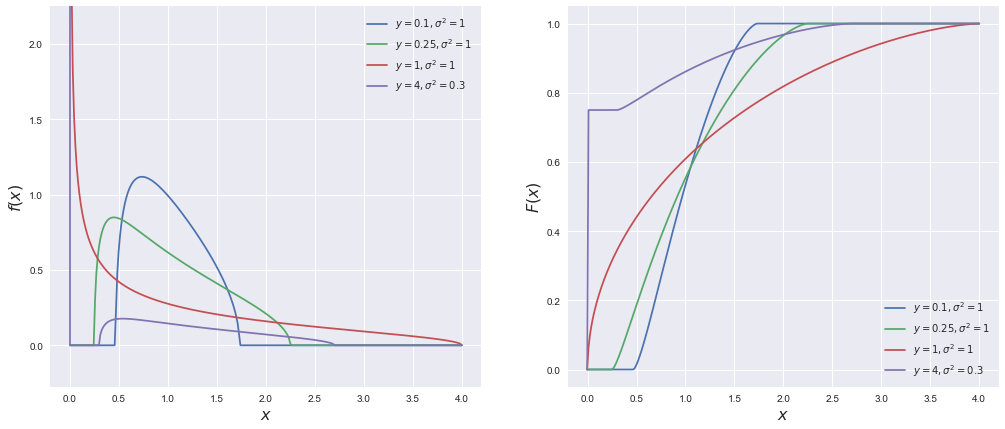
\includegraphics[scale=0.4]{MP}
			\caption{Marchenko-Pastur law}
		\end{center}
	\end{figure}
	
	\section*{Non-constant volatility case}
	\begin{rmrk}
		Let us set
		\[ \Theta_t^0 = \sqrt{\int_0^1\Theta_s^2 ds} \quad \forall t \in [0, 1] \]
		and corresponding matrix $\mathbf{X}_t^0$, such that
		\[ d\mathbf{X}_t^0 = \Theta_t^0d\mathbf{W}_t. \]
		Note that $\mathbf{X}_t$ and $\mathbf{X}_t^0$ share the same ICV matrix:
		\[ \Sigma_p^0 :=  \int_0^1(\Theta_t^0)^2 dt = \int_0^1 dt \int_0^1 \Theta_s^2 ds = \Sigma_p.  \]
		Based on $\mathbf{X}_t^0$, we have an associated RCV matrix
		\[ \Sigma_p^{RCV^0} = \sum_{\ell=1}^{n} \Delta \mathbf{X}_\ell^0 (\Delta \mathbf{X}_\ell^0)^T. \]
		Since $\Sigma_p^{RCV}$ and $\Sigma_p^{RCV^0}$ are based on the same estimation method and share the same targeting ICV matrix, it is desirable that their ESDs have similar properties. \\
		... bla bla bla discuss convergence and conclude that we can show that RCV may not converge in non-constant volatility case.
	\end{rmrk}
	
	\begin{defn}
		Let $A$, $B$ be two symmetric $p \times p$ matrices. Then we write
		\[ A \succeq B\]
		to denote that $A-B$ is a positive semidefinite matrix. Similarly, we say that $A \preceq B$ if $A-B$ is negative semidefinite.
	\end{defn}
	
	\begin{lmm}[Weyl's Monotonicity Theorem]
		Suppose $A$ and $B$ are symmetric, $p \times p$ matrices. Let $\lambda_i(A)$ be the $i$-th largest eigenvalue of $A$. If $A \preceq B$, then $\lambda_i(A) \leq \lambda_i(B)$ for all $i$, or, equivalently
		\[ F^B(x) \leq F^A(x) \quad \forall x \geq 0. \]
    \end{lmm}
    \begin{proof}
    	Corollary 4.3.3 in Horn and Johnson (1990).
    \end{proof}
		
	\begin{prps} \label{counter RCV}
		Suppose that for all $p$, $\mathbf{X}_t=\mathbf{X}_t^{(p)}$ is a $p$-dimensional process satisfying
		\begin{equation}
		d \mathbf{X}_t = \gamma_t d\mathbf{W}_t, \quad t \in [0, 1],
		\end{equation}
		where $\gamma_t > 0$ is a nonrandom (scalar) c$\grave{\text{a}}$dl$\grave{\text{a}}$g process. Let $\sigma^2 = \int_0^1 \gamma_t^2 dt$ and so that the ICV matrix $\Sigma_p = \sigma^2 \mathbb{I}_{p \times p}$. Assume further that the observation times $\tau_{\ell}$ are equally spaced, that is, $\tau_{\ell} = \ell / n$, and that the RCV matrix $\Sigma_p^{RCV}$ is defined by \eqref{RCV}. Then so long as $\gamma_t$ is not constant on $[0, 1)$, for any $\varepsilon > 0$, there exists $y_c = y_c(\gamma, \varepsilon) > 0$ such that if $\lim p/n = y \geq y_c$,
		\begin{equation}
			\limsup F^{\Sigma_p^{RCV}}(b(y)+\sigma^2\varepsilon) < 1 \quad \text{a.s.}
		\end{equation}
		In particular, $F^{\Sigma_p^{RCV}}$ doesn't converge to the Marchenko-Pastur law $\mathcal{MP}(y, \sigma^2)$.
    \end{prps}
    
    \begin{proof}
    	By assumption if $\gamma_t$ is non-contant, there exists $\delta > 0$ and an interval $[c, d] \subseteq [0, 1] $ such that
    	\[ \gamma_t \geq \sigma(1+\delta) \quad \forall t \in [c, d]. \]
    	Therefore, if $\big[ \frac{\ell - 1}{n}, \frac{\ell}{n} \big] \subseteq [c, d] $ for some $1 \leq \ell \leq n$, then
    	\[ \Delta \mathbf{X}_\ell (\Delta \mathbf{X}_\ell )^T \stackrel{d}{=} \int_{(\ell-1)/n}^{\ell/n} \gamma_t^2 dt \cdot \mathbf{Z}_\ell(\mathbf{Z}_\ell)^T \succeq \frac{(1+\delta)^2}{n} \sigma^2 \mathbf{Z}_\ell(\mathbf{Z}_\ell)^T,  \]
    	where $\mathbf{Z}_\ell = (Z_\ell^{(1)}, \dots , Z_\ell^{(p)})^T$ consists of independent standard normals. Hence, if we let $ J_n = \big\{ \ell: \big[ \frac{\ell - 1}{n}, \frac{\ell}{n} \big] \subseteq [c, d] \big\} $ and
    	\[ \Gamma_p = \sum_{\ell \in J_n} \Delta \mathbf{X}_\ell (\Delta \mathbf{X}_\ell )^T, \quad \Lambda_p = \frac{\sigma^2}{n(d-c)} \sum_{\ell \in J_n} \mathbf{Z}_\ell (\mathbf{Z}_\ell )^T,  \]
    	then for any $x \geq 0$, by Weyl's Monotonicity Theorem,
    	\[
    	F^{\Sigma_p^{RCV}}(x) \leq F^{\Gamma_p}(x) \leq F^{\Lambda_p}\bigg(\frac{x}{(1+\delta)^2(d-c)}\bigg).
    	\]
	    Now note that $\# J_n \sim (d-c)n$, hence if $p/n \rightarrow y$, by Proposition \ref{MP law}, $F^{\Lambda_p}$ will converge a.s. to the Marchenko-Pastur law with ratio index $y'=\frac{y}{d-c}$ and scale index $\sigma^2$.
	    By the formula of $b(\cdot)$ in Marchenko-Pastur density
	    \[
	    \begin{aligned}
	    (1+\delta)^2(d-c)b(y') &=(1+\delta)\sigma^2 \cdot (1+\delta)(d-c)(1+2\sqrt{y'}+y') \\
	    & =(1+\delta)\sigma^2 \cdot (1+\delta)(d-c + 2\sqrt{(d-c)y} + y) \\
	    & := (1+\delta)\sigma^2 \cdot  g(y).
	    \end{aligned}
	    \]
	    Note that the $g(y)$ has a linear growth in $y$ with coefficient $1+\delta$. Hence, for any $\varepsilon > 0$, there exists $y_c > 0$, such that for all $y \geq y_c$
	    \[ g(y) \geq (1+\sqrt{y})^2+\varepsilon,  \]
	    that is,
	    \[ (1+\delta)^2(d-c)b(y') \geq (1+\delta) \sigma^2 \cdot ((1+\sqrt{y})^2+\varepsilon) = (1+\delta)(b(y)+\sigma^2\varepsilon)  \]
	    or, equivalently,
	    \[ \frac{b(y) + \sigma^2\varepsilon}{(1+\delta)^2(d-c)} \leq \frac{b(y')}{1+\delta}. \]
	    Therefore, when the above inequality holds,
	    \[\limsup F^{\Sigma_p^{RCV}}(b(y) + \sigma^2\varepsilon) \leq \limsup F^{\Lambda_p}\bigg(\frac{b(y')}{1+\delta}\bigg) < 1. \]
    \end{proof}
    
    \pagebreak
    \part{Limit theorems for non-constant covolatility processes}
    
    \section*{Limiting distribution for realized covariance}
    \begin{rmrk}
    	In this part we will state two major theorems. The first one is a generalization of Proposition \ref{MP law} for limiting spectral distribution of RCV matrix in the case of non-constant covolatility. The second theorem claims the convergence of ESD of alternative estimator to Marchenko-Pastur law. Both theorems require some additional assumptions.
    \end{rmrk}
    
    \begin{thm} \label{Thm 1}
    	Assume that all the conditions in Proposition \ref{MP law} are satisfied. Furthermore,
    	\begin{enumerate}
    		\item $Z_\ell^{(p, j)}$ have finite moments of all orders;
    		\item $H$ has a finite second moment;
    		\item the weights $w_\ell^n$, $1 \leq \ell \leq n$, $n = 1, 2, \dots$, are all positive, and there exists $\kappa < \infty$ such that the rescaled weights $(nw_\ell^n)$ satisfy
    		\[ \max_n \max_{\ell = 1, \dots, n} (nw_\ell^n) \leq \kappa; \]
    		moreover, almost surely, there exists a c$\grave{\text{a}}$dl$\grave{\text{a}}$g function $w_s: [0, 1] \rightarrow \MR_{+}$, such that
    		\[ \lim_n \sum_{1 \leq \ell \leq n} \int_{(\ell-1)/n}^{\ell/n} |n w_\ell^n - w_s|ds = 0; \]
    		\item there exists a sequence $\eta_p = o(p)$ and a sequence of index sets $\mathcal{I}_p$ satisfying $\mathcal{I}_p \subset \{1, \dots, p\}$ and $\#\mathcal{I}_p \leq \eta_p$ such that for all $n$ and all $\ell$, $w_\ell^n$ may depend on $\mathbf{Z}_\ell^{(p)}$ but only on $\{ Z_\ell^{(p,j)}: j \in \mathcal{I}_p \}$;
    		\item there exist $C < \infty$ and $\delta < 1/6$ such that for all $p$, $\| \Sigma_p \| \leq Cp^\delta$ a.s.
    	\end{enumerate}
    	Define $S_p = \sum_{\ell=1}^{n} w_\ell^n \cdot \Sigma_p^{1/2} \mathbf{Z}_\ell^{(p)} (\mathbf{Z}_\ell^{(p)})^T\Sigma_p^{1/2} $. Then, almost surely, the ESD of $S_p$ converges in distribution to a probability distribution $F^w$, which is determined by $H$ and $(w_s)$ in that its Stiltjes trasform $m_{F^w}(z)$ is given by
    	\[ m_{F^w}(z) = -\frac{1}{z} \int_{\tau \in \MR} \frac{1}{\tau M(z) + 1} dH(\tau), \]
    	where $M(z)$, together with another function $\tilde{m}(z)$, uniquely solve the following equation in $\mathbb{C}_{+} \times \mathbb{C}_{+}$:
    	\[
    	\left \{
    	\begin{array}{l}
    		M(z) = -\frac{1}{z} \int_{\tau \in \MR} \frac{w_s}{1 + y \tilde{m}(z)w_s} ds,  \\
    		\tilde{m}(z) =  -\frac{1}{z} \int_{\tau \in \MR} \frac{\tau}{\tau M(z) + 1} dH(\tau).
    	\end{array}
    	\right.
    	\]
    \end{thm}
    
    \begin{rmrk}
    	If $w_\ell^n = 1/n$, then $w_s=1$, and Theorem \ref{Thm 1} reduces to Proposition \ref{MP law}. Moreover, if $w_s$ is not constant, that is, $w_s \neq \int_{0}^{1} w_t dt$ on $[0, 1]$, then except in the trivial case when $H$ is a delta measure at $0$, the LSD $F^w \neq F$, where $F$ is the LSD in Proposition \ref{MP law} determined by $H(\cdot / \int_{0}^{1} w_t dt)$. (ADD MORE EXPLANATION FROM SUPPLEMENTARY ARTICLE)
    \end{rmrk}
    
    \section*{Time-variance adjusted realized covariance}
    
    \begin{defn}
   		Suppose that $\mathbf{X}_t$ is a $p$-dimensional process satisfying \eqref{X diffeq}, and $\Theta_t$ is c$\grave{\text{a}}$dl$\grave{\text{a}}$g. We say that $\mathbf{X}_t$ belongs to \define{class $\mathcal{C}$} if, almost surely, there exist $\gamma_t: [0, 1] \mapsto \MR$ and $\Lambda$ a $p \times p$ matrix satisfying $\tr(\Lambda \Lambda^T) = p$ such that 
   		\begin{equation} \label{class C cov}
   		\Theta_t = \gamma_t \Lambda.
   		\end{equation}
   		Observe that if \eqref{class C cov} holds, then the ICV matrix $\Sigma_p = \int_{0}^{1} \gamma_t^2 dt \cdot \Lambda \Lambda^T$. The special case when $\Lambda = \mathbb{I}_{p \times p}$ is studied in the next part.
   	\end{defn}
    		
    \begin{exmp}
    	Suppose that $X_t^{(j)}$ satisfy
    		\[ dX_t^{(j)} = \mu_t^{(j)} dt + \sigma_t^{(j)}dW_t^{(j)}, \quad j = 1, \dots, p, \]
    		where $\mu_t^{(j)}, \sigma_t^{(j)} : [0, 1] \rightarrow \MR$ are the drift and volatility processes for stock $j$, and $W_t^{(j)}$'s are (one-dimensional) standard Brownian motions. If the following conditions hold:
    		\begin{itemize}
    			\item the correlation matrix process of $(W_t^{(j)})$
    			\[ R_t:= \bigg(\frac{ [W^{(j)}, W^{(k)}]_t \ }{t}\bigg)_{1 \leq j,k \leq p} =:(r^{(jk)})_{1 \leq j,k \leq p} \]
    			is constant in $t \in [0, 1]$.
    			\item $r^{(jk)} \neq 0$ for all $1 \leq j,k \leq p$; and
    			\item the correlation matrix process of $X_t^{(j)}$
    			\[ \Bigg( \frac{\int_{0}^{t} \sigma_s^{(j)}\sigma_s^{(k)} d[W^{(j)}, W^{(k)}]_s }{\sqrt{\int_{0}^{t} (\sigma_s^{(j)})^2 ds \cdot \int_{0}^{t} (\sigma_s^{(k)})^2 ds}} \Bigg)_{1 \leq j,k \leq p}  =:(\rho^{(jk)})_{1 \leq j,k \leq p}  \]
    			is constant in $t \in [0, 1]$;
    		\end{itemize}
    		then $\mathbf{X}_t$ belongs to class $\mathcal{C}$.
    		
    		\begin{proof}
    			For any $t \in [0, 1]$: 
    			\[ \rho^{(jk)} = \frac{r^{(jk)} \int_{0}^{t} \sigma_s^{(j)}\sigma_s^{(k)} ds }{\sqrt{\int_{0}^{t} (\sigma_s^{(j)})^2 ds \cdot \int_{0}^{t} (\sigma_s^{(k)})^2 ds}}, \]
    			therefore
    			\[ \frac{\rho^{(jk)}}{r^{(jk)}} = \frac{\int_{0}^{t} \sigma_s^{(j)}\sigma_s^{(k)} ds/t }{\sqrt{\int_{0}^{t} (\sigma_s^{(j)})^2 ds/t \cdot \int_{0}^{t} (\sigma_s^{(k)})^2 ds/t}}. \]
    			Letting $t \downarrow 0$, using l'H$\hat{\text{o}}$pital's rule and noting that $\sigma_t^{(j)}$ are c$\grave{\text{a}}$dl$\grave{\text{a}}$g, we observe that
    			\[ \frac{\rho^{(jk)}}{r^{(jk)}} = \frac{\sigma_0^{(j)}\sigma_0^{(k)}}{ \sqrt{  (\sigma_0^{(j)})^2 \cdot (\sigma_0^{(k)})^2 }} = \pm 1. \]
    			Hence, for all $t \in [0, 1]$:
    			\[ \bigg| \int_{0}^{t}\sigma_s^{(j)}\sigma_s^{(k)} ds \bigg| = \sqrt{\int_{0}^{t} (\sigma_s^{(j)})^2 ds \cdot \int_{0}^{t} (\sigma_s^{(k)})^2 ds} . \]
    			By Cauchy-Schwartz inequality, this holds only if $\sigma_s^{(j)}$ and $\sigma_s^{(k)}$ are proportional to each other. Therefore, almost surely, there exists a scalar process $\gamma_t : [0, 1] \rightarrow \MR$ and a $p$-dimensional vector $(\sigma^{(1)}, \dots, \sigma^{(p)})^T$, such that
    			\[ (\sigma_t^{(1)}, \dots, \sigma_t^{(p)})^T = \gamma_t \cdot (\sigma^{(1)}, \dots, \sigma^{(p)})^T. \]
    			Now we show that $\mathbf{X}_t$ belongs to class $\mathcal{C}$. In fact one can always find a $p$-dimensional standard Brownian motion $\widetilde{\mathbf{W}}_t$, such that 
    			\[ \mathbf{W}_t = R^{1/2}\widetilde{\mathbf{W}}_t, \]
    			where $\mathbf{W} = (W_t^{(1)}, \dots, W_t^{(p)})^T$ and $R$ is a correlation matrix of $\mathbf{W}_t$, which is constant for all $t \in [0, 1]$ by assumption. Hence, writing $\mu_t = (\mu_t^{(1)}, \dots, \mu_t^{(p)})^T$, we have
    			\[ d\mathbf{X}_t = \mu_t dt + \diag(\sigma_t^{(1)}, \dots, \sigma_t^{(p)}) d\mathbf{W}_t = \mu_t dt +\gamma_t \cdot \diag(\sigma^{(1)}, \dots, \sigma^{(p)}) R^{1/2} d\widetilde{\mathbf{W}}_t. \]
    		\end{proof}
    \end{exmp}
    
    \begin{rmrk}
    	The process in Example \ref{exmp X3} doesn't belong to the class $\mathcal{C}$, because its correlation structure varies in time.
    \end{rmrk}
    		
    \begin{defn}
   		Suppose that a diffusion process $\mathbf{X}_t$ belongs to class $\mathcal{C}$. We define \define{time-variation adjusted realized covariance (TVARCV) matrix} as follows:
   		\begin{equation} \label{TVARCV}
   		\widehat{\Sigma}_p := \frac{\tr \big( \Sigma_p^{RCV} \big) }{n} \sum_{\ell = 1}^{n} \frac{\Delta \mathbf{X}_\ell (\Delta \mathbf{X}_\ell)^T}{\| \Delta \mathbf{X}_\ell \|_2^2} = \frac{\tr \big( \Sigma_p^{RCV} \big) }{p} \widetilde{\Sigma}_p,
   		\end{equation}
   		where
   		\begin{equation} \label{Sigma_tilde}
   		\widetilde{\Sigma}_p := \frac{p}{n} \sum_{\ell = 1}^{n} \frac{\Delta \mathbf{X}_\ell (\Delta \mathbf{X}_\ell)^T}{\| \Delta \mathbf{X}_\ell \|_2^2}.
   		\end{equation}
    \end{defn}
    
    \begin{rmrk}
    	Let us explain $\widetilde{\Sigma}_p$. Consider the simplest case when $\mu_t = 0$, $\gamma_t$ deterministic, $\Lambda_t = \mathbb{I}_{p \times p}$, and $\tau_{\ell} = \ell / n$, $\ell = 0, 1, \dots, n$. In this case,
    	\[ \Delta \mathbf{X}_\ell = \sqrt{\int_{(\ell - 1)/n}^{\ell / n} \gamma_t^2 dt }\cdot \frac{\mathbf{Z}_\ell}{\sqrt{n}}, \]
    	where $\mathbf{Z}_\ell = (Z_\ell^{(1)}, \dots, Z_\ell^{(p)})^T$ is a vector of i.i.d. standard normal random variables. Hence,
    	\[ \frac{\Delta \mathbf{X}_\ell (\Delta \mathbf{X}_\ell)^T}{\| \Delta \mathbf{X}_\ell \|_2^2} = \frac{\mathbf{Z}_\ell \mathbf{Z}_\ell^T}{\|  \mathbf{Z}_\ell \|_2^2}. \]
    	However, as $p \rightarrow \infty$, $\| \mathbf{Z}_\ell \|_2^2 \sim p$, hence
    	\[ \widetilde{\Sigma}_p \sim \frac{\sum_{\ell = 1}^{n}\mathbf{Z}_\ell \mathbf{Z}_\ell^T}{n}, \]
    	the latter being the usual sample covariance matrix.
    	We will show that, first, $\tr(\Sigma_p^{RCV}) \sim \tr(\Sigma_p)$; and second, if $\mathbf{X}_t$ belongs to class $\mathcal{C}$ and satisfies certain additional assumptions, then the LSD of $\widetilde{\Sigma}_p$ is related to that of $\breve{\Sigma}_p$ via the Marchenko-Pastur equation, where
    	\[ \breve{\Sigma}_p = \frac{p}{\tr(\Sigma_p)}\Sigma_p = \Lambda \Lambda^T. \]
    	Hence, the LSD of $\widehat{\Sigma}_p$ is also related to that of $\Sigma_p$ via the same Marchenko-Pastur equation.
    	We will now state our assumptions for the major theorem in this paper.
    \end{rmrk}
    
    \begin{asmp} \label{asmp2} \
    	\begin{enumerate}
    		\item there exists $C_0 < \infty$ such that for all $p$ and all $j = 1, \dots, p$, $|\mu_t^{(p,j)}| \leq C_0$ for all $t \in [0, 1]$ a.s.;
    		\item there exist constants $C_1 < \infty$, $0 \leq \delta_1 < 1/2$, a sequence $\eta_p < C_1 p^{\delta_1}$ and a sequence of index sets $\mathcal{I}_p$ satisfying $\mathcal{I}_p \subset \{ 1, \dots p \}$ and $\# \mathcal{I}_p \leq \eta_p$ such that $\gamma_t^{(p)}$ may depend on $\mathbf{W}_t^{(p)}$ but only on $\{ W_t^{(p, j)} : j \in \mathcal{I}_p \}$; moreover, there exists $C_2 < \infty$ such that for all $p$, $|\gamma_t^{(p)}| \in (1/C_2, C_2)$ for all $t \in [0, 1]$ a.s.;
    		\item there exists $C_3 < \infty$ such that for all $p$ and for all $j$, the individual volatilities \[ \sigma_t^{(j)} = \gamma_t^{(p)}\sqrt{\sum_{k=1}^{p} (\Lambda_{jk}^{(p)})^2} \in (1/C_3, C_3)\] for all $t \in [0, 1]$ a.s.;
    		\item \[ \lim_{p \rightarrow \infty} \frac{\tr(\Sigma_p)}{p} = \lim_{p \rightarrow \infty} \int_{0}^{1} (\gamma_t^{(p)})^2 dt := \theta > 0 \quad \text{a.s.}; \]
    		\item almost surely, as $p \rightarrow \infty$, the ESD $F^{\Sigma_p}$ converges to a probability distribution $H$ on $[0, \infty)$;
    		\item there exist $C_5 < \infty$ and $0 \leq \delta_2 < 1/2$ such that for all $p$, $\| \Sigma_p \| \leq C_5 p^{\delta_2}$ a.s.;
    		\item the $\delta_1$ in (ii) and $\delta_2$ in (vi) satisfy that $\delta_1 + \delta_2 < 1/2$;
    		\item $p/n \rightarrow y \in (0, \infty) $ as $p \rightarrow \infty$; and
    		\item there exists $C_4 < \infty$ such that for all $n$,
    		\[ \max_{1 \leq \ell \leq n} n \cdot (\tau_{\ell} - \tau_{\ell - 1}) \leq C_4 \quad \text{a.s.}  \]
    		moreover, $\tau_{\ell}$'s are independent of $\mathbf{X}_t$.
    	\end{enumerate}
    \end{asmp}
    
    \begin{rmrk}
    	Before stating and proving theorem for TVARCV we provide some useful lemmas.
    \end{rmrk}
    
    \begin{lmm}[Burkholder-Davis-Gundy inequality] \label{BDG}
    	For any real number $p \geq 1$ there exist positive constants $c_p$ and $C_p$ such that, for all local martingales $X_t$ with $X_0 = 0$, its maximum processes $M_t = \sup_{t \leq s} |X_s|$ and stopping times $\tau$, the following inequalities hold
    	\[ c_p \ME[[X]_\tau^{p/2}] \leq \ME[M_\tau^p] \leq C_p \ME[[X]_\tau^{p/2}]. \]
    \end{lmm}
    \begin{proof}
    	LOOK IN THE BOOKS
    \end{proof}
    
    \begin{lmm} \label{lmm1}
    	Suppose that for each $p$, $\mathbf{v}_\ell^{(p)} = (v_\ell^{p, 1}, \dots, v_\ell^{(p, p)})^T$ and $\mathbf{w}_\ell^{(p)} = (w_\ell^{(p, 1)}, \dots, w_\ell^{(p, p)})^T$, $\ell = 1, \dots, n$, are all $p$-dimensional vectors. Define
    	\[	\widetilde{S}_n = \sum_{\ell = 1}^{n} (\mathbf{v}_\ell^{(p)} + \mathbf{w}_\ell^{(p)}) \cdot (\mathbf{v}_\ell^{(p)} + \mathbf{w}_\ell^{(p)})^T\]
    	and
    	\[S_n = \sum_{\ell = 1}^{n} \mathbf{w}_\ell^{(p)} (\mathbf{w}_\ell^{(p)})^T. \]
    	If the following conditions are satisfied:
    	\begin{enumerate}
    		\item $\lim_{p \rightarrow \infty} p/n = y > 0$;
    		\item there exists a sequence $\varepsilon_p = o(1/\sqrt{p})$ such that for all $p$ and all $\ell$, all the entries of $\mathbf{v}_\ell^{(p)}$ are bounded by $\varepsilon_p$ in absolute value;
    		\item $ \limsup_{p \rightarrow \infty} {\tr(S_n)}/{p} < \infty$ almost surely.
    	\end{enumerate}
    	Then $L(F^{\widetilde{S}_n}, F^{S_n}) \rightarrow 0$ almost surely, where for any two probability distribution functions $F$ and $G$
    	\[ L(F, G) := \inf \{ \varepsilon > 0 : F(x-\varepsilon) -\varepsilon \leq G(x) \leq F(x+\varepsilon) + \varepsilon \quad \forall x\in\MR   \} \]
    	denotes the L$\acute{\text{e}}$vy distance between them.
    \end{lmm}
    \begin{proof}
    	
    \end{proof}
    
    \begin{prps}
    	Under Assumptions \ref{asmp2}(iv), namely, suppose that
    	\[ \lim_{p \rightarrow \infty} \frac{\tr(\Sigma_p)}{p} = \theta \quad \text{a.s.}, \]
    	then
    	\[ \lim_{p \rightarrow \infty} \frac{\tr(\Sigma_p^{RCV})}{p} = \theta \quad \text{a.s.} \]
    \end{prps}
    \begin{proof}
    	The full proof can be found in supplementary article. We will provide here the main idea:
    \end{proof}
    
    \begin{thm} \label{Thm 2}
    	Suppose that for all $p$, $\mathbf{X}_t = \mathbf{X}_t^{(p)}$ is a $p$-dimensional process in class $\mathcal{C}$ for some drift process $\mu_t^{(p)} = (\mu_t^{(p, 1)}, \dots , \mu_t^{(p, p)})^T$, covolatility process $\Theta_t^{(p)} = \gamma_t^{(p)} \Lambda^{(p)}$ and a $p$-dimensional Brownian motion $\mathbf{W}_t^{(p)}$, which satisfy Assumptions \ref{asmp2} (i)-(vii) above. Suppose also that $p$ and $n$ satisfy Assumption \ref{asmp2} (viii), and the observation times satisfy Assumption \ref{asmp2}(ix). Let $\hat{\Sigma}_p$ be as in \eqref{TVARCV}. Then, as $p \rightarrow \infty$, $F^{\hat{\Sigma}_p}$ converges a.s. to a probability distribution $F$, which is determined by $H$ through Stieltjes transforms via the same Marchenko-Pastur equation as in Proposition \ref{MP law}.
    \end{thm}
    \begin{proof}
    	First we state that both $F^{\breve{\Sigma}_p}$ and $F^{\widetilde{\Sigma}_p}$ converge almost surely. $F^{\breve{\Sigma}_p}$ converges to $\breve{H}$, which is defined by
    	\[\breve{H}(x) = H(\theta x) \quad \forall x \geq 0.  \]
    	The LSD $\widetilde{F}$ of $\widetilde{\Sigma}_p$ is determined by $\breve{H}$ in that its Stieltjes transform $m_{\widetilde{F}}(z)$ satisfies the equation
    	\[ m_{\widetilde{F}}(z) = \int_{\tau \in \MR} \frac{1}{ \tau(1- y(1 + zm_{\widetilde{F}}(z))) - z } d\breve{H}(\tau). \]
    	The convergence of $F^{\breve{\Sigma}_p}$ is obvious since
    	\[ F^{\breve{\Sigma}_p} = F^{\Sigma_p}(\tr(\Sigma_p)/p \cdot x) \quad \forall x \geq 0.  \]
    	We now show the convergence of $F^{\Sigma_p}$. First, note that
    	\[ \Delta \mathbf{X}_\ell = \int_{\tau_{\ell-1}}^{\tau_\ell} \boldsymbol{\mu}_t dt + \Lambda \cdot \int_{\tau_{\ell-1}}^{\tau_\ell} \gamma_t d\mathbf{W}_t := \sqrt{\int_{\tau_{\ell-1}}^{\tau_\ell} \gamma_t^2 dt}\cdot (\mathbf{v}_\ell + \Lambda \cdot \mathbf{Z}_\ell), \]
    	where
    	\[ \mathbf{v}_\ell = (v_\ell^{(1)}, \dots, v_\ell^{(p)})^T = \frac{\int_{\tau_{\ell-1}}^{\tau_\ell} \boldsymbol{\mu}_t dt}{\sqrt{\int_{\tau_{\ell-1}}^{\tau_\ell} \gamma_t^2 dt}} \]
    	and
    	\[ \mathbf{Z}_\ell = (Z_\ell^{(1)}, \dots, Z_\ell^{(p)})^T = \frac{\int_{\tau_{\ell-1}}^{\tau_\ell} \gamma_t d\mathbf{W}_t}{\sqrt{\int_{\tau_{\ell-1}}^{\tau_\ell} \gamma_t^2 dt}} \]
    	By performing an orthogonal transformation if necessary, w.l.o.g., we may assume that the index set $\mathcal{I}_p \subset \{ 1, \dots, \eta_p \} $. Then by Assumptions \ref{asmp2} (ii) and (ix), for $j > \eta_p$, $Z_\ell^{(j)}$ are i.i.d. $\sim \mathcal{N}(0, 1)$. Write
    	\[ \mathbf{U}_\ell = (Z_\ell^{(1)}, \dots Z_\ell^{(\eta_p)})^T \]
    	and 
    	\[ \mathbf{D}_\ell = (Z_\ell^{(\eta_p+1)}, \dots Z_\ell^{(p)})^T.\]
    	With the above notation, $\widetilde{\Sigma}_p$ can be rewritten as
    	\begin{equation}
    	\widetilde{\Sigma}_p = y_n \sum_{\ell=1}^{n} \frac{\Delta \mathbf{X}_\ell (\Delta \mathbf{X}_\ell)^T}{\|\Delta \mathbf{X}_\ell\|_2^2} = y_n \sum_{\ell=1}^{n} \frac{(\mathbf{v}_\ell + \Lambda \mathbf{Z}_\ell) (\mathbf{v}_\ell + \Lambda \mathbf{Z}_\ell)^T}{\|\mathbf{v}_\ell + \Lambda \mathbf{Z}_\ell\|_2^2}
    	\end{equation}
    	By Assumptions \ref{asmp2} (i), (ii) and (ix), there exists $C > 0$, such that $|v_\ell^{(j)}| \leq C / \sqrt{n}$ for all $j$ and $\ell$, hence $\| \mathbf{v}_\ell\|_2$'s are uniformly bounded. We will show that
    	\begin{equation} \label{334}
    		\max_{\ell = 1, \dots, n} \Bigg|\frac{  \| \Lambda \mathbf{Z}_\ell \|_2^2}{p} - 1\Bigg| = \max_{\ell = 1, \dots, n} \Bigg| \frac{  \mathbf{Z}_\ell^T \breve{\Sigma}_p \mathbf{Z}_\ell}{p} - 1\Bigg| \rightarrow 0 \quad \text{a.s.},
    	\end{equation}
    	which clearly implies that
    	\begin{equation} \label{335}
    		\max_{\ell = 1, \dots, n} \Bigg|\frac{  \| \mathbf{v}_\ell + \Lambda\mathbf{Z}_\ell  \|_2^2}{p} - 1\Bigg| \rightarrow 0 \quad \text{a.s.}
    	\end{equation}
    	To prove \eqref{334} let us write
    	\[ \breve{\Sigma}_p = \begin{pmatrix}
    	A & B \\
    	B^T & C
    	\end{pmatrix}, \]
    	where $A$, $B$ and $C$ are $\eta_p \times \eta_p$, $\eta_p \times (n - \eta_p)$ and $(n-\eta_p) \times (n-\eta_p)$ matrices, respectively. Then
    	\[ \mathbf{Z}_\ell^T \breve{\Sigma}_p \mathbf{Z}_\ell = \mathbf{U}_\ell^T A \mathbf{U}_\ell + 2\mathbf{D}_\ell^T B^T \mathbf{U}_\ell + \mathbf{D}_\ell^T C \mathbf{D}_\ell.  \]    	
    	By a well-known fact about the spectral norm,
    	\[ \|A\| \leq \|\breve{\Sigma}_p \|, \quad \|B\| \leq \|\breve{\Sigma}_p \| \quad \text{and} \quad \|C\| \leq \|\breve{\Sigma}_p \|. \]
    	In particular, by Assumptions \ref{asmp2} (ii), (vi) and (vii),
    	\[ 0 \leq \tr(A) \leq \eta_p \cdot \|\breve{\Sigma}_p \| \leq Cp^{\delta_1 + \delta_2} = o(p), \]
    	hence 
    	\[ \frac{\tr(C)}{p} = \frac{\tr(\breve{\Sigma}_p)-\tr(A)}{p} \rightarrow 1. \]
    	Now using the fact that $\mathbf{D}_\ell$ consists of i.i.d. standard normals and by the same proof as that for (READ THE PROOF AND WRITE IT HERE!!!)
    	we get
    	\[ \max_{\ell = 1, \dots, n} \Bigg| \frac{\mathbf{D}_\ell^T C \mathbf{D}_\ell}{p} - 1 \Bigg| \rightarrow 0 \quad \text{a.s.} \]
    	To complete the proof of \eqref{334}, it then suffices to show that
    	\[ \max_{\ell = 1, \dots, n} \frac{| \mathbf{U}_\ell^T A \mathbf{U}_\ell |}{p} \rightarrow 0 \quad \text{and} \quad \max_{\ell = 1, \dots, n} \frac{| \mathbf{D}_\ell^T B \mathbf{U}_\ell |}{p} \rightarrow 0 \quad \text{a.s.} \]
    	We shall only prove the first convergence, the second one can be proved similarly. We have
    	\begin{equation} \label{337}
    		|\mathbf{U}_\ell A \mathbf{U}_\ell| \leq \|A\| \cdot \|\mathbf{U}_\ell\|_2^2 \leq C_5 p^{\delta_2} \cdot \|\mathbf{U}_\ell\|_2^2
    	\end{equation}
    	Observe that for all $1 \leq i \leq \eta_p$, by Assumptions \ref{asmp2} (ii),
    	\[ | Z_\ell^{(i)} |^2 = \frac{|\int_{\tau_{\ell-1}}^{\tau_\ell} \gamma_t d\mathbf{W}_t|^2}{\int_{\tau_{\ell-1}}^{\tau_\ell} \gamma_t^2 dt} \leq \frac{C_2^2}{\tau_\ell-\tau_{\ell-1} } \cdot \Bigg|\int_{\tau_{\ell-1}}^{\tau_\ell} \gamma_t d\mathbf{W}_t \Bigg|^2. \] 
    	By Lemma \ref{BDG} , we then get that for any $k \in \MN$, there exists $\lambda_k > 0$ such that
    	\begin{equation} \label{338}
    		\ME[ |Z_\ell^{(i)}|^{2k} ] \leq \lambda_k C_2^{4k}.
    	\end{equation}
    	Now we are ready to show that $\max_{\ell = 1, \dots, n} \frac{| \mathbf{U}_\ell^T A \mathbf{U}_\ell |}{p} \rightarrow 0 $. In fact, for any $\varepsilon > 0$, for any $k \in \MN$, by Markov's inequality\footnote{
    		Markov's inequality states that for any non-negative random variable $X$, $k \in \MN$ and $n \in \MR_+$ the following inequality holds:
    		\[ \MP(X \geq n) \leq \frac{\ME[X^k]}{n^k}. \]
    		}, \eqref{337}, H\"older's inequality and \eqref{338},
    	\[ 
    	\begin{aligned}
    	\MP(\max_{\ell = 1, \dots, n} | \mathbf{U}_\ell^T A \mathbf{U}_\ell | \geq p\varepsilon) & \leq \sum_{\ell=1}^{n} \MP(|\mathbf{U}_\ell^T A \mathbf{U}_\ell | \geq p\varepsilon) \\
    	& \leq \sum_{\ell=1}^{n} \frac{\ME[ |\mathbf{U}_\ell^T A \mathbf{U}_\ell|^k ]}{ p^k \varepsilon^k } \\
    	& \leq \sum_{\ell=1}^{n} \frac{ C_5^k p^{k \delta_2}  \cdot \eta_p \cdot \lambda_k C_2^{4k} \cdot \eta_p^{k-1} }{p^k\varepsilon^k} \\
    	& \leq C p^{1+k\delta_2 + k\delta_1 - k}.
    	\end{aligned}
    	 \]
    	 By Assumptions \ref{asmp2} (vii), $\delta_1 + \delta_2 < 1/2$, hence by choosing $k$ to be large enough, the right hand side will be summable in $p$: 
    	 \[ \sum_{p=1}^{\infty} \MP\big(\max_{\ell = 1, \dots, n} | \mathbf{U}_\ell^T A \mathbf{U}_\ell | \geq p\varepsilon\big) < \infty. \]
    	 Hence by Borel–Cantelli lemma\footnote{
    	 	Let $X_1, X_2, \dots$ be a sequence of random variables in some probability space and $\varepsilon > 0$ be arbitrary.
    	 	Then
    	 	\[ \sum_{n=1}^{\infty} \MP(|X_n| \geq \varepsilon) < \infty \Longrightarrow X_n \xrightarrow{a.s.} 0.  \]
    	 	}, almost surely, $\max_{\ell = 1, \dots, n} \frac{| \mathbf{U}_\ell^T A \mathbf{U}_\ell |}{p} \rightarrow 0$.
    	 We now get back to $\widetilde{\Sigma}_p$. By \eqref{335}, for any $\varepsilon > 0$, almost surely, for all $n$ sufficiently large, for all $\ell = 1, \dots, n$,
    	 \[ p(1-\varepsilon) \leq \| \mathbf{v}_\ell + \Lambda \mathbf{Z}_\ell \|_2^2 \leq p(1+\varepsilon). \]
    	 Hence, almost surely, for all $n$ sufficiently large,
    	 \[ \frac{1}{1+\varepsilon} \widetilde{S}_p \preceq \widetilde{\Sigma}_p = y_n \sum_{\ell=1}^{n} \frac{(\mathbf{v}_\ell + \Lambda \mathbf{Z}_\ell) (\mathbf{v}_\ell + \Lambda \mathbf{Z}_\ell)^T}{\|\mathbf{v}_\ell + \Lambda \mathbf{Z}_\ell\|_2^2} \preceq \frac{1}{1-\varepsilon} \widetilde{S}_p, \]
    	 where
    	 \[  \widetilde{S}_p = \frac{1}{n}\sum_{\ell=1}^{n} (\mathbf{v}_\ell + \Lambda \mathbf{Z}_\ell) (\mathbf{v}_\ell + \Lambda \mathbf{Z}_\ell)^T. \]
    	 Hence, by Weyl's Monotonicity theorem,
    	 \begin{equation} \label{339}
    	     F^{\widetilde{S}_p}((1+\varepsilon)x) \geq F^{\widetilde{\Sigma}_p}(x) \geq F^{\widetilde{S}_p}((1-\varepsilon)x) \quad \forall x \geq 0.
    	 \end{equation}
    	 Next, by Lemma \ref{lmm1} $\widetilde{S}_p$ has the same LSD as 
    	 \[S_p := \frac{1}{n} \sum_{\ell=1}^{n} \Lambda \mathbf{Z}_\ell (\mathbf{Z}_\ell)^T \Lambda^T.\]
    	 Moreover, by using the same trick as in the beginning of the proof of THEOREM 1 (WHICH TRICK???), $F^{S_p}$ has the same limit as $F^{S'_p}$, where
    	 \[S'_p := \frac{1}{n} \sum_{\ell=1}^{n} \Lambda \widetilde{\mathbf{Z}}_\ell (\widetilde{\mathbf{Z}}_\ell)^T \Lambda^T\]
    	 and $\widetilde{\mathbf{Z}}_\ell$ consists of i.i.d. standard normals. For $F^{S'_p}$, it follows easily from Proposition \ref{MP law} that it converges to $\widetilde{F}$. Moreover, by BY SOME THEOREMS IN THIS F** BOOKS, $\widetilde{F}$ is differentiable and in particular continuous at all $x > 0$. It follows from \eqref{339} that $F^{\widetilde{\Sigma}_p}$ must also converge to $\widetilde{F}$.
    \end{proof}
    
    \pagebreak
    \part{Simulation studies}
    \section*{Non-equidistant observation times}
    \begin{exmp} \label{SimCos}
    	Let's take an example from the paper...
    	\[
    		\gamma_t = \sqrt{0.0009 + 0.0008 \cos(2 \pi t)}.
    	\]
    	Then
    	\[ \sigma^2 = 0.0009 + \int_{0}^{1}0.0008 \cos(2 \pi t) dt = 0.0009. \]
    \end{exmp}
    
    \begin{figure}
    	\begin{center} \centering
    		\includegraphics[scale=0.4]{XCos2}
    		\caption{ $\mathbf{X_t}$ from Example \ref{SimCos}, $n = 1000$, $p=4000$, $\sigma^2 = 0.0009$ }
    		\smallskip
    		\small
    		In this setting $y = p/n = 4$. Note point mass equal to $0.75$ at the origin. Also note, that the domain of $F^{RCV}$ is larger than the domain of Marchenko-Pastur law, as it was proved in Proposition \ref{counter RCV}.
    	\end{center}
    \end{figure}
    
    \begin{exmp} \label{PosTimes}
    	Let us set time points $ \{\tau_\ell\}_{0 \leq \ell \leq n}$, where $\tau_0 = 0$ a.s. and interarrival times are independent and obey the exponential distribution with rate $\lambda$, that is 
    	\[ \MP(\tau_{\ell} - \tau_{\ell-1} > x) =  e^{-\lambda x}, \quad 1 \leq \ell \leq n. \]
    	Then by Strong Law of Large Numbers
    	\[ \frac{\tau_n}{n} = \frac{1}{n} \sum_{\ell=1}^{n} (\tau_{\ell} - \tau_{\ell-1}) \xrightarrow{a.s.} \ME[\tau_1] = \lambda. \]
    	Define
    	\[ \mathcal{T} = \{\tau_\ell : \tau_\ell \in [0, 1]\}, \]
    	then by setting $\lambda = \frac{1}{n}$, we get $\#\mathcal{T} \sim n$.
    	Let's take volatility $\gamma_t$ as in Example \ref{SimCos}.
    \end{exmp}
    
    \begin{figure}
    	\begin{center} \centering
    		\includegraphics[scale=0.4]{XCos}
    		\caption{ $\mathbf{X_t}$ from Example \ref{SimCos}, $n = 1000$, $p=1000$ }
    		\smallskip
    		\small
    		In this setting $y = p/n = 1$...
    	\end{center}
    \end{figure}
    
    \begin{figure}
    	\begin{center} \centering
    		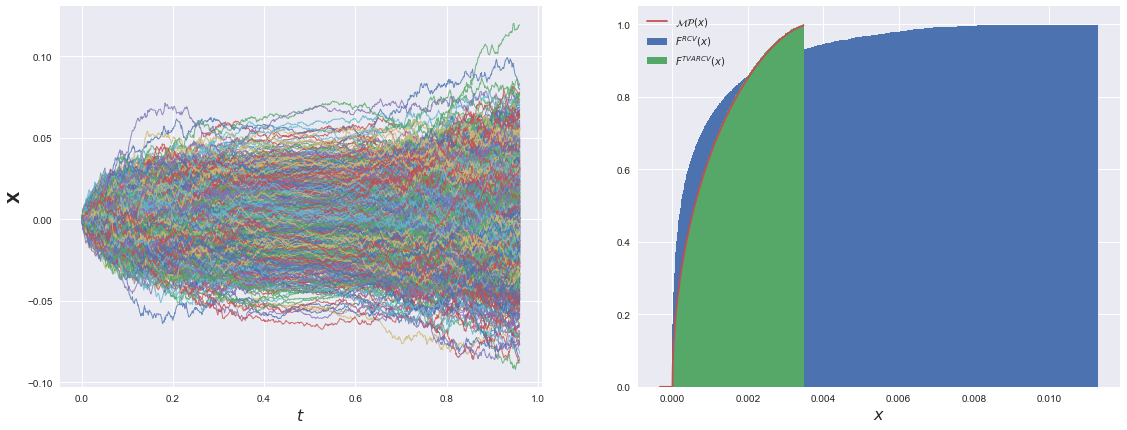
\includegraphics[scale=0.4]{Xcostimes}
    		\caption{ $\mathbf{X_t}$ from Example \ref{PosTimes}, $n \simeq 1000$, $p=1000$ }
    		\smallskip
    		\small
    		We see that if observation times are not equidistant, the ESD of RCV changes drastically, even if visually there is no difference in realizations of $\mathbf{X}_t$.
    	\end{center}
    \end{figure}
    
    
    \section*{Stochastic volatility case}
    \begin{defn} \
    	\begin{enumerate}
    		\item 
    		The stochastic process $Y_t$ is called \define{Cox-Ingersoll-Ross (CIR) process}, if it is determined by the stochastic differential equation (SDE):
    		\begin{equation} \label{CIR}
    		    dY_t = \beta(\alpha - Y_t)dt + \xi\sqrt{Y_t}d \overline{W}_t,
    		\end{equation}
    		where $\alpha$, $\beta$ and $\xi$ are positive constants, and $\overline{W}_t$ is a standard Brownian motion. Conditional on parameters and initial value $Y_0$, scaled CIR process has a non-central chi-squared distribution with $k$ degrees of freedom and non-centrality parameter $\lambda$:
    		\[ c Y_t \sim {\chi'}_k^2(\lambda),  \]
    		where
    		\[k = \frac{4\alpha \beta}{\xi^2},\ \lambda = Y_0 c e^{-\beta t} \ \text{and} \ c = \frac{4 \beta}{\xi^2 (1-e^{-\beta t})}.\]
    		CIR process never goes below $0$. Moreover, it is a.s. positive if the condition
    		\[ 2\alpha \beta \geq \xi^2  \]
    		is met. This property makes CIR process a perfect tool for volatility (or interest rate) modeling.
    		\item The standard \define{Heston model} assumes that one-dimensional log-price process $X_t$ is determined by the following SDE:
    		\begin{equation}
    		dX_t = \mu dt + \sqrt{Y_t}d{W}_t,
    		\end{equation}
    		where $Y_t$ satisfies SDE \eqref{CIR} and ${W}_t$ is another standard Brownian motion, such that 
    		\begin{equation} \label{dependent Brownian}
    		[{W}, \overline{W}]_t = \int_{0}^{t}\rho_s ds
    		\end{equation}
    		holds with a (stochastic) process $\rho_t$, taking values strictly between $-1$ and $1$. Sometimes equality \eqref{dependent Brownian} is informally written as
    		\[ d{W}_td\overline{W}_t = \rho_t dt. \]
    	\end{enumerate}
    \end{defn}
    
    \begin{exmp} \label{SimCIR}
    	Let's assume
    	\[ \gamma_t = \sqrt{Y_t}, \]
    	where $Y_t$ is a CIR process, determined by \eqref{CIR}. Then it is easy to show that
    	\[ \sigma^2 = \beta\alpha - \beta\int_{0}^{1} \gamma_t^2dt + \xi \int_{0}^{1} \gamma_t d\overline{W}_t.\]
    	Therefore, as long as $\xi > 0$, the value of $\sigma^2$ is random and for different realizations of $\gamma_t$ we have different LSD.
    	Moreover, let
    	\[ \overline{W}_t = \frac{1}{\sqrt{\eta_p}} \sum_{j=1}^{\eta_p}W_t^{(j)}, \]
    	where $\eta_p$ is determined by Assumption \ref{asmp2} (ii). The process $\overline{W}_t$ is still the standard Brownian motion, because it is a.s. continuous, has independent increments and
    	\[ \overline{W}_t - \overline{W}_s = \frac{1}{\sqrt{\eta_p}} \sum_{j=1}^{\eta_p}(W_t^{(j)}-W_s^{(j)}) \sim \mathcal{N}(0, t-s) \quad \forall t < s. \]
    	We also take $\eta_p = p$, that means that $\overline{W}_t$ is a sample average of $\mathbf{W}_t$ and depends on every its component $W_t^{(j)}$. Simulations show that even in this case, when Assumptions \ref{asmp2} (ii) are not satisfied, Theorem \ref{Thm 2} still holds and $F^{TVARCV}$ converges to Marchenko-Pastur law. Intuitively it can be explained in the following way:
    	For any $0 \leq i \leq p$ we have
    	\[ dW_t^{(i)}\cdot d\overline{W}_t = dW_t^{(i)} \cdot \frac{1}{\sqrt{\eta_p}} \sum_{j=1}^{\eta_p}dW_t^{(j)} = \frac{dt}{\sqrt{\eta_p}} \mathbf{1}_{\{i \leq \eta_p\}}, \]
    	or equivalently 
    	\[ [W^{(i)}, \overline{W}]_t =  \frac{t}{\sqrt{\eta_p}} \mathbf{1}_{\{i \leq \eta_p\}}.  \]
    	Hence, with growing $\eta_p$ the dependence of $\overline{W}_t$ on ... becomes smaller and for $\eta_p = p \rightarrow \infty$ correlation between them goes to $0$.
    \end{exmp}
    
    \begin{figure}
    	\begin{center} \centering
    		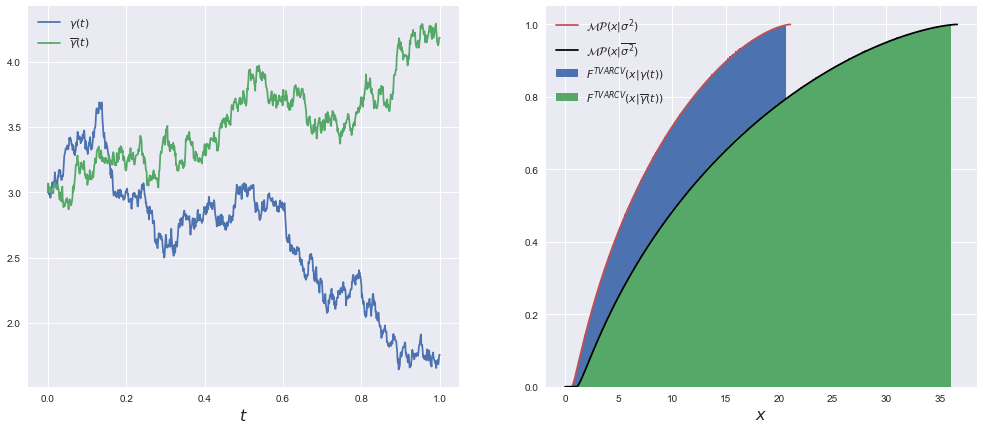
\includegraphics[scale=0.4]{XCIR}
    		\caption{$\eta_p = p, y = 0.5, \alpha = 5, \beta = 1, \gamma_0 = 3, \xi = 2$}
    		\smallskip
    		\small
    		We see that even with the same parameters of volatility model, we have the different scale parameter in asymptotic spectral distribution.
    	\end{center}
    \end{figure}
    
    \section*{Jump-diffusion processes}
    \begin{rmrk}
    	(CHECK TEXT HERE!)
    	Before we discussed pure diffusion processes, namely that these processes are continuous almost sure. It is quite useful to consider so-called jump-diffusion processes... How should we change our estimator then?
    	ALSO MENTION ONE- AND FINITE-DIMENSIONAL PROCESSES, THEN GO FOR P->INF
    	ALSO WE ONLY CONSIDER EQUIDISTANT TIMES
	    AND ONLY SIGMA EQUAL TO IDENTITY, WHICH MEANS INDPENENCE
	    AND MU = 0
    \end{rmrk}
    
    \begin{exmp} \label{uniform jumps} \
    	\begin{enumerate}
    	\item Simplest model: let $U \sim \mathcal{U}[0, 1]$ be standard uniformly distributed random variable and
    	\begin{equation}
    	d\mathbf{X}_t = \gamma_t  d\mathbf{W}_t + \Delta_U(t),
    	\end{equation}
    	where $\Delta_U(t) = (\delta_U(t), \dots, \delta_U(t))^T$ is a vector of Dirac delta functions shifted to $U$. In other words, all the components of $\mathbf{X}_t$ make a jump of size $1$ at the same random time $t = U$. Let us denote by $\mathbf{X^c}_t$ the continuous part of $\mathbf{X}_t$. Moreover, let $\ell'$ denote the index of interval, where $U$ is located:
    	\[ U \in \bigg[\frac{\ell'-1}{n}, \frac{\ell'}{n}\bigg). \]
    	Then
    	\[ 
    	\begin{aligned}
    	\Sigma_p^{RCV} & = \sum_{\ell=1, \ell \neq \ell'}^{n}\Delta \mathbf{X}_\ell(\Delta \mathbf{X}_\ell)^T + \Delta \mathbf{X}_{\ell'}(\Delta \mathbf{X}_{\ell'})^T\\
    	 & = \sum_{\ell=1, \ell \neq \ell'}^{n}\Delta \mathbf{X}_\ell(\Delta \mathbf{X}_\ell)^T + (\Delta \mathbf{X^c}_{\ell'} + \mathbb{U}_{p \times 1})(\Delta \mathbf{X^c}_{\ell'} + \mathbb{U}_{p \times 1})^T\\
    	& =  \sum_{\ell=1}^{n}\Delta \mathbf{X^c}_\ell(\Delta \mathbf{X^c}_\ell)^T + \Delta \mathbf{X^c}_{\ell'} \cdot \mathbb{U}_{1 \times p} + (\Delta \mathbf{X^c}_{\ell'} \cdot \mathbb{U}_{1 \times p})^T + \mathbb{U}_{p \times p} ,
    	\end{aligned}
    	\]
    	where $\mathbb{U}_{k \times j}$ stands for $k \times j$ matrix filled with ones. Note that the elements of $\Delta \mathbf{X^c}_{\ell'} \cdot \mathbb{U}_{1 \times p}$ are i.i.d. $ \sim \mathcal{N}\big(0, \Gamma_{\ell'}/n )$ with $\Gamma_{\ell'}=\int_{(\ell' - 1)/n}^{\ell' / n} \gamma_t^2 dt$. Therefore, if we set $n \rightarrow \infty$, $\tr(\Sigma_p^{RCV})$ will converge to the same value as before plus $p$. Also,
    	\[
    	\| \Delta \mathbf{X}_{\ell'} \|_2^2 = \| \Delta \mathbf{X^c}_{\ell'} + \mathbb{U}_{p \times 1} \|_2^2  = \sum_{j=1}^{p} (\Delta X^c_{\ell'})^2 + 2\sum_{j=1}^{p} \Delta X^c_{\ell'} + p.
    	\]
    	We have asymptotically:
    	\[
    	 \sum_{j=1}^{p} (\Delta X^c_{\ell'})^2 \sim \frac{p}{n}\Gamma_{\ell'}
    	 \]
    	 as a sum of $p$ i.i.d. normally distributed random variables with variance $\Gamma_{\ell'}/n$ and
    	 \[ \sum_{j=1}^{p} \Delta X^c_{\ell'} \sim \mathcal{N}\Big(0, \frac{p}{n}\Gamma_{\ell'}\Big). \]
    	 As long as $p/n$ converges to some finite constant, $\Gamma_{\ell'}$ is bounded and $p$ converges to infinity, we have
    	 \[ 
    	 \frac{\Delta \mathbf{X}_{\ell'}(\Delta \mathbf{X}_{\ell'})^T}{\| \Delta \mathbf{X}_{\ell'} \|_2^2} \rightarrow 0.
    	  \]
    	  Hence, if we know that all components jumped at the same time and the size of the jump is equal to $1$, new estimator will be
    	  \[ 
    	  \Sigma_p^{TVARCV} = \frac{\tr(\Sigma_p^{RCV}) - p}{n} \sum_{\ell=1}^{n} \frac{\Delta \mathbf{X}_{\ell}(\Delta \mathbf{X}_{\ell})^T}{\| \Delta \mathbf{X}_{\ell'} \|_2^2}.
    	   \]
   	
    	\item Now let $U_1, \dots, U_p$ be i.i.d. $\sim \mathcal{U}[0, 1]$, $\mathbf{U} = (U_1, \dots, U_p)^T$ and
    	\[ 
    	d\mathbf{X}_t = \gamma_t  d\mathbf{W}_t + \Delta_\mathbf{U}(t)
        \]
        with $\Delta_\mathbf{U}(t) = (\delta_{U_1}(t), \dots, \delta_{U_p}(t))^T$.
        \end{enumerate}
    \end{exmp}
    
    \begin{rmrk}
    	In Example \ref{uniform jumps} we assumed that in the interval $[0, 1]$ each component of the process $\mathbf{X}_t$ had exactly one jump. In practice, jump-diffusion processes are often modeled using Poisson processes, where one cannot be sure how many jumps can happen in given interval.
    \end{rmrk}
    
    \begin{defn} \
    	\begin{enumerate}
    		\item To construct a Poisson process, we begin with a sequence of arrival times $\tau_1^N, \tau_2^N, \dots$, where
    		\[ \tau_{j+1}^N - \tau_j^N \sim \operatorname{Exp}(\lambda) \quad \forall j \geq 1.  \]
    		This setting is similar to the one in Example \ref{PosTimes}, except that now $\tau_j^N$ stands for the time of $j$-th jump. \define{The Poisson process} $N(t)$ counts the number of jumps that occur at or before time $t$. More precisely,
    		\[ N(t) = \sum_{j \geq 1} \mathbf{1}_{ \{\tau_j^N \leq t\}}. \]
    		Because the expected time between jumps is $1/\lambda$, the jumps are arriving at an average rate of $\lambda$ per unit time. We say the Poisson process $N(t)$ has intensity $\lambda$.
    		\item Let $N(t)$ be a Poisson process with intensity $\lambda$, and let $Y_1, Y_2, \dots$ be a sequence of i.i.d. random variables with mean
    		\[ \beta = \ME[Y_1]. \]
    		We assume the random variables $Y_1, Y_2, \dots$ are also independent of $N(t)$. We define the \define{compound Poisson process}
    		\[ Q(t) = \sum_{i=1}^{N(t)} Y_i, \quad t \geq 0. \]
    		The jumps in $Q(t)$ occur at the same times as the jumps in $N(t)$, but whereas the jumps in $N(t)$ are always of size $1$, the $j$-th jump in $Q(t)$ is of random size $Y_j$.
    	\end{enumerate}
    \end{defn}
    
    \pagebreak
    \part{Conclusion}
    
\end{document}
